\chapter{Recurrent Neural Networks}

Up until now, we considered feedforward neural networks. The input is read from the first layer, then traverses a number of hidden layers, and the prediction is finally produced by the output layer. Recurrent neural networks are a different category of architecture, based on the addition of feedback loops to the network topology. These self loops provide the network with dynamical properties, introducing the ability of holding a memory (state) of past computations of the model.

RNNs have been the reference approach for sequence processing, especially for speech and text recognition, processing, and generation. The type of data handled by these models is structured; it is usually an ordered set of sequences of vectors.

\section{Memory}

The introduction of feedback loops allows the network to hold a memory about past computations. This memory is needed because the output of a certain input depends on previous outputs produced by the same network.
\begin{figure}[h]
    \centering
    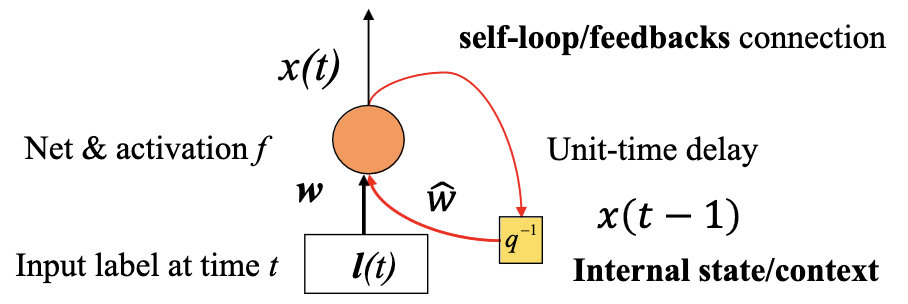
\includegraphics[width=0.5\linewidth]{img/RNN_unit.png}
\end{figure}

The output of the node is calculated for a time $t$ recursively, as:
\begin{equation*}
    x(t) = \begin{cases}
            0 & t = 0 \\
            \tau(i(t), x(t-1)) = f(w^Ti(t) + \hat{w}x(t-1) + \theta) & t \geq 0 \\
    \end{cases}
\end{equation*}
Here, $f$ is the activation function of the unit, $i(t)$ is the input label at time $t$, $\hat{w}$ is the recurrent weight (the one that's coming from a feedback), and $\theta$ is the bias. The internal state summarizes the past information, and changes each time the unit produces a new output. The encoding of the past memory is also adaptive. $\tau$ is the state transition function realized by the NN. $x(t)$ here refers only to one state, but it can also include a set of states.

\section{Properties}

Many RNN architectures are possible, but even a simple one with a few nodes each with its own feedback loop is already incredibly powerful. They are universal approximators of non-linear dynamic systems, and are Turing equivalent (they can simulate any automata).

RNN models are based on the following assumptions:
\begin{itemize}
    \item \textbf{Causality}: a system is causal if the output at time $t_0$ only depends on inputs at time $t<t_0$ (necessary and sufficient for internal state);

    \item \textbf{Stationarity}: time invariance after model training. The state transition function $\tau$ is independent on node $v$ of the sequence.

    \item \textbf{Adaptivity}: transition functions are realized by NN with free parameters, so they are learned from data.
\end{itemize}

RNNs can also be \textbf{unfolded}. Unfolding a RNN means representing it as a graph with a repetitive structure corresponding to a chain of events (so it represents how the same model behaves through time). Unfolding is associated with weight sharing between unfolded layers. The learning algorithms used for RNNs must account the set of encode transitions developed by the model for each step of the inputs. \textbf{Backpropagation through time (BPTT)} and \textbf{real time recurrent learning (RTRL)} are two supervised learning algorithms designed for RNNs that compute gradient values of the output errors across an unfolded network.

An approach related to RNNs are \textbf{transformers}. A transformer is a deep learning architecture that relies on a mechanism called \textbf{attention}, which allows the model to access any preceding point along the sequence. The attention layer weighs all previous states according to some learned measure of relevance. This method is especially useful for language translation, where the context of the whole sentence (given by all the previous words) is important to define the meaning of a word.

\section{Echo State Networks}

Echo State Networks are an emerging paradigm for efficiently modeling RNNs. An ESN consists of:
\begin{itemize}
    \item A \textbf{reservoir} of sparsely connected recurrent units, untrained after a \textbf{random initialization};

    \item Simple feedforward readout of linear units, trained by efficient linear methods.
\end{itemize}
They are efficient in the sense that they don't need any training of the recurrent units, and yet they're capable of easily solving certain tasks (under specific conditions). The reservoir acts as a projection of the input sequences into values belonging to a state space. Different input sequences are discriminated on a suffix-based fashion with no training needed: the closeness between states is proportional to the length of their common suffix.

RNNs can be extended to rooted trees, as \textbf{Recursive Neural Networks}. 